\chapter{Financial Study}
\epigraph{\textit{"The first rule is to never lose money. The second rule is to never forget the first one."}}{Warren Buffett} 

The different departments have estimated the main costs of the project. It is high time to start performing a deep analysis on the economical solvency of the project. The analysis carried on will be of 12 years. The decision of this amount of years has been done taking into account that every 5 years there is a re-launching of the whole constellation, which means a considerable increase in the costs. In order to have a good view of the whole project, it has been decided that at least two full cycles had to appear complete (years 0 to 4 and 5 to 9) and also to see the tendency it was recommended to add some more time. This is the reason why the studied is carried on for 12 years.

From an analysis carried on by Astrea's team, it has been found that the anual estimation of the demand can be approximated by 295650000 Mbits hired per year. An economical study is going to be performed using that estimation as the sales. The determination of the price of Astrea'a service is made upon this feasibility study. 

When performing the feasibility study, all the costs must be taken into account. This means that all the costs derived from the different departments (communications, satellites, launching, ...) are considered, as well as other costs such as the engineering hours, which were stated in the Project Charter and the Gantt Chart. All those costs have already been explained. Nevertheless, some last costs which must be taken into account are the administration costs and the insurance service. The estimations of those costs are of 259000 and 2245320 \euro  per year, respectively. For further details on the studies mentioned, please refer to the [{REF TO ANNEX: Anex V. Section 11}].  All the costs can be found in the Budget as well.


\newgeometry{left=2cm,right=3cm}

\begin{landscape}
\centering
\begin{table}[]
\vspace*{\fill}
\resizebox{\columnwidth}{!}{%
\begin{tabular}{| l | l | l | l | l | l | l | l | l | l | l | l | l | l |}
\hline
\rowcolor[gray]{0.65}
\textbf{TIME}                                                                          & \textbf{Year 0}  & \textbf{Year 1} & \textbf{Year 2} & \textbf{Year 3} & \textbf{Year 4} & \textbf{Year 5} & \textbf{Year 6} & \textbf{Year 7} & \textbf{Year 8} & \textbf{Year 9} & \textbf{Year 10} & \textbf{Year 11} & \textbf{Year 12} 
\\ \hline
\rowcolor[gray]{0.85}
\textbf{INVESTMENT (build GS)}                                                         & \textbf{-4,07}   &                 &                 &                 &                 &                 &                 &                 &                 &                 &                  &                  &                  \\
\hline
\rowcolor[gray]{0.85}
\textbf{INCOME}                                                                        &                  &                 &                 &                 &                 &                 &                 &                 &                 &                 &                  &                  &                  \\
Percentage (learning curve)                                                            &                  & 0,75            & 0,80            & 0,85            & 0,90            & 0,95            & 1,00            & 1,00            & 1,00            & 1,00            & 1,00             & 1,00             & 1,00             \\
Number of Mbits hired                                                                  &                  & 4,435E+07       & 4,730E+07       & 5,026E+07       & 5,322E+07       & 5,617E+07       & 5,913E+07       & 5,913E+07       & 5,913E+07       & 5,913E+07       & 5,913E+07        & 5,913E+07        & 5,913E+07        \\
Gain (M euros)                                                                         &                  & 44,35           & 47,30           & 50,26           & 53,22           & 56,17           & 59,13           & 59,13           & 59,13           & 59,13           & 59,13            & 59,13            & 59,13            \\
\textbf{Total Income}                                                                  & \textbf{0,00}    & \textbf{44,35}  & \textbf{47,30}  & \textbf{50,26}  & \textbf{53,22}  & \textbf{56,17}  & \textbf{59,13}  & \textbf{59,13}  & \textbf{59,13}  & \textbf{59,13}  & \textbf{59,13}   & \textbf{59,13}   & \textbf{59,13}   
\\ \hline
\rowcolor[gray]{0.85}
\textbf{COSTS}                                                                         &                  &                 &                 &                 &                 &                 &                 &                 &                 &                 &                  &                  &                  \\
n planes/year                                                                          & 9                &                 &                 &                 &                 & 9               &                 &                 &                 &                 & 9                & 0                & 0                \\
Satellites/year                                                                        & 189              & 0               & 0               & 0               & 0               & 189             & 0               & 0               & 0               & 0               & 189              & 0                & 0                \\
\textbf{Engineering hours}                                                             & -0,0395          &                 &                 &                 &                 &                 &                 &                 &                 &                 &                  &                  &                  \\
\textbf{Administration}                                                                &                  & -0,259          & -0,259          & -0,259          & -0,259          & -0,259          & -0,259          & -0,259          & -0,259          & -0,259          & -0,259           & -0,259           & -0,259           \\
\textbf{Insurance}                                                                     &                  & -2,24532        & -2,24532        & -2,24532        & -2,24532        & -2,24532        & -2,24532        & -2,24532        & -2,24532        & -2,24532        & -2,24532         & -2,24532         & -2,24532         \\
\textbf{\begin{tabular}[c]{@{}l@{}}Web hosting, maint. and\\   promotion\end{tabular}} & -0,005           & -0,005          & -0,005          & -0,005          & -0,005          & -0,005          & -0,005          & -0,005          & -0,005          & -0,005          & -0,005           & -0,005           & -0,005           \\
\textbf{Launching}                                                                     &                  &                 &                 &                 &                 &                 &                 &                 &                 &                 &                  &                  &                  \\
Planes                                                                                 & -48,256          & 0,000           & 0,000           & 0,000           & 0,000           & -48,256         & 0,000           & 0,000           & 0,000           & 0,000           & -48,256          & 0,000            & 0,000            \\
Satellites                                                                             & -3,024           & 0,000           & 0,000           & 0,000           & 0,000           & -3,024          & 0,000           & 0,000           & 0,000           & 0,000           & -3,024           & 0,000            & 0,000            \\
\textbf{System (satellites)}                                                           &                  &                 &                 &                 &                 &                 &                 &                 &                 &                 &                  &                  &                  \\
\textit{Assembly (individual)}                                                         & -3,78            & 0,00            & 0,00            & 0,00            & -3,78           & 0,00            & 0,00            & 0,00            & 0,00            & -3,78           & 0,00             & 0,00             & 0,00             \\
\textit{Assembly (constellation)}                                                      & -0,15            & 0,00            & 0,00            & 0,00            & -0,15           & 0,00            & 0,00            & 0,00            & 0,00            & -0,15           & 0,00             & -0,15            & -0,15            \\
Structure                                                                              & -0,737           & 0,000           & 0,000           & 0,000           & -0,74           & 0,000           & 0,000           & 0,000           & 0,000           & -0,74           & 0,000            & 0,000            & 0,000            \\
Thermal protection                                                                     & -0,189           & 0,000           & 0,000           & 0,000           & -0,19           & 0,000           & 0,000           & 0,000           & 0,000           & -0,19           & 0,000            & 0,000            & 0,000            \\
\textit{Electric power system}                                                         &                  &                 &                 &                 &                 &                 &                 &                 &                 &                 &                  &                  &                  \\
Solar arrays                                                                           & -12,852          & 0,000           & 0,000           & 0,000           & -12,85          & 0,000           & 0,000           & 0,000           & 0,000           & -12,85          & 0,000            & 0,000            & 0,000            \\
Batteries                                                                              & -2,381           & 0,000           & 0,000           & 0,000           & -2,38           & 0,000           & 0,000           & 0,000           & 0,000           & -2,38           & 0,000            & 0,000            & 0,000            \\
Power management                                                                       & -3,024           & 0,000           & 0,000           & 0,000           & -3,02           & 0,000           & 0,000           & 0,000           & 0,000           & -3,02           & 0,000            & 0,000            & 0,000            \\
\textit{Payload}                                                                       &                  &                 &                 &                 &                 &                 &                 &                 &                 &                 &                  &                  &                  \\
Patch antenna                                                                          & -12,663          & 0,000           & 0,000           & 0,000           & -12,66          & 0,000           & 0,000           & 0,000           & 0,000           & -12,66          & 0,000            & 0,000            & 0,000            \\
Antenna deployment                                                                     & -0,567           & 0,000           & 0,000           & 0,000           & -0,57           & 0,000           & 0,000           & 0,000           & 0,000           & -0,57           & 0,000            & 0,000            & 0,000            \\
Transciever inter-satellite                                                            & -4,845           & 0,000           & 0,000           & 0,000           & -4,85           & 0,000           & 0,000           & 0,000           & 0,000           & -4,85           & 0,000            & 0,000            & 0,000            \\
Transciever space to ground                                                            & -1,040           & 0,000           & 0,000           & 0,000           & -1,04           & 0,000           & 0,000           & 0,000           & 0,000           & -1,04           & 0,000            & 0,000            & 0,000            \\
Data handling system                                                                   & -0,945           & 0,000           & 0,000           & 0,000           & -0,95           & 0,000           & 0,000           & 0,000           & 0,000           & -0,95           & 0,000            & 0,000            & 0,000            \\
Variable expenses                                                                      & -0,756           & 0,000           & 0,000           & 0,000           & -0,76           & 0,000           & 0,000           & 0,000           & 0,000           & -0,76           & 0,000            & 0,000            & 0,000            \\
\textit{AOCDS}                                                                         &                  &                 &                 &                 &                 &                 &                 &                 &                 &                 &                  &                  &                  \\
Thruster                                                                               & -9,450           & 0,000           & 0,000           & 0,000           & -9,45           & 0,000           & 0,000           & 0,000           & 0,000           & -9,45           & 0,000            & 0,000            & 0,000            \\
CubeSpace ACDS                                                                         & -2,835           & 0,000           & 0,000           & 0,000           & -2,84           & 0,000           & 0,000           & 0,000           & 0,000           & -2,84           & 0,000            & 0,000            & 0,000            \\
\textbf{Communications}                                                                &                  &                 &                 &                 &                 &                 &                 &                 &                 &                 &                  &                  &                  \\
Maintenance GS Canada                                                                  &                  & -0,011          & -0,011          & -0,011          & -0,011          & -0,011          & -0,011          & -0,011          & -0,011          & -0,011          & -0,011           & -0,011           & -0,011           \\
Maintenance GS Scotland (UK)                                                           &                  & -0,015          & -0,015          & -0,015          & -0,015          & -0,015          & -0,015          & -0,015          & -0,015          & -0,015          & -0,015           & -0,015           & -0,015           \\
Maintenance GS Malvines                                                                &                  & -0,015          & -0,015          & -0,015          & -0,015          & -0,015          & -0,015          & -0,015          & -0,015          & -0,015          & -0,015           & -0,015           & -0,015           \\
Maintenance MCC                                                                        &                  & -0,029          & -0,029          & -0,029          & -0,029          & -0,029          & -0,029          & -0,029          & -0,029          & -0,029          & -0,029           & -0,029           & -0,029           \\
Salaries GS Canada                                                                     &                  & -0,382          & -0,382          & -0,382          & -0,382          & -0,382          & -0,382          & -0,382          & -0,382          & -0,382          & -0,382           & -0,382           & -0,382           \\
Salaries GS Scotland (UK)                                                              &                  & -0,226          & -0,226          & -0,226          & -0,226          & -0,226          & -0,226          & -0,226          & -0,226          & -0,226          & -0,226           & -0,226           & -0,226           \\
Salaries GS Malvines                                                                   &                  & -0,082          & -0,082          & -0,082          & -0,082          & -0,082          & -0,082          & -0,082          & -0,082          & -0,082          & -0,082           & -0,082           & -0,082           \\
Salaries MCC                                                                           &                  & -0,430          & -0,430          & -0,430          & -0,430          & -0,430          & -0,430          & -0,430          & -0,430          & -0,430          & -0,430           & -0,430           & -0,430           \\
Licenses                                                                               &                  & -0,010          & -0,010          & -0,010          & -0,010          & -0,010          & -0,010          & -0,010          & -0,010          & -0,010          & -0,010           & -0,010           & -0,010           \\
\textbf{Total Cost}                                                                    & \textbf{-107,54} & \textbf{-3,71}  & \textbf{-3,71}  & \textbf{-3,71}  & \textbf{-59,92} & \textbf{-54,99} & \textbf{-3,71}  & \textbf{-3,71}  & \textbf{-3,71}  & \textbf{-59,92} & \textbf{-54,99}  & \textbf{-3,86}   & \textbf{-3,86}   
\\ \hline \hline
\rowcolor[gray]{0.85}
\textbf{CASH FLOW}                                                                     & \textbf{-111,61} & \textbf{40,64}  & \textbf{43,60}  & \textbf{46,55}  & \textbf{-6,71}  & \textbf{1,19}   & \textbf{55,42}  & \textbf{55,42}  & \textbf{55,42}  & \textbf{-0,79}  & \textbf{4,14}    & \textbf{55,27}   & \textbf{55,27}   \\
\rowcolor[gray]{0.85}
\textbf{DISC CF}                                                                       & \textbf{-111,61} & \textbf{38,34}  & \textbf{38,80}  & \textbf{39,09}  & \textbf{-5,31}  & \textbf{0,89}   & \textbf{39,07}  & \textbf{36,86}  & \textbf{34,77}  & \textbf{-0,47}  & \textbf{2,31}    & \textbf{29,12}   & \textbf{27,47}   \\
\rowcolor[gray]{0.85}
\textbf{CUM CF}                                                                        & \textbf{-111,61} & \textbf{-70,97} & \textbf{-27,37} & \textbf{19,18}  & \textbf{12,47}  & \textbf{13,66}  & \textbf{69,08}  & \textbf{124,50} & \textbf{179,92} & \textbf{179,13} & \textbf{183,27}  & \textbf{238,54}  & \textbf{293,82}  \\
\rowcolor[gray]{0.85}
\textbf{DIS CUM CF}                                                                    & \textbf{-111,61} & \textbf{-73,27} & \textbf{-34,47} & \textbf{4,62}   & \textbf{-0,69}  & \textbf{0,19}   & \textbf{39,26}  & \textbf{76,12}  & \textbf{110,89} & \textbf{110,42} & \textbf{112,74}  & \textbf{141,85}  & \textbf{169,32} 
\\ \hline
\end{tabular}
}
\vspace*{\fill}
\caption{Feasibility Study}
\label{Feasibility Study}
\end{table}
\end{landscape}

\restoregeometry

\begin{itemize}
\item Pay Back Time: The Cumulative Cash Flow is plotted next. It can be seen that the Pay Back Time is between years 2 and 3. Assuming linearly distributed, it will be of 2.68 years. The value of the first PBT (2.63 years) found seems reasonably acceptable, taking into account that this project requires a great budget, as all space projects do, due to its own nature. In year 4, the satellites that are going to be launched in year 5 are made. This means an increase in the cost, due to the fabrication and assembly. Moreover, in year 5, there is also a increase, even more significant, because of the re-launching itself of those satellites. This is what causes that interval of time in which the Cumulative Cash Flow does not increase, but even decreases a bit: that year, the income is slighly smaller than the re-launching costs. A second Pay Back Time might be found of 5.05 years. Since the investment was done in year 4, it means an actual Pay Back Time of 1.05 years, for the second investment. In years 9 and 10, the same process takes place again: the fabrication and re-launching of the new satellites. Nevertheless, profit is high enough at this point so that the Cumulative Cash Flow does not get to negative values again.

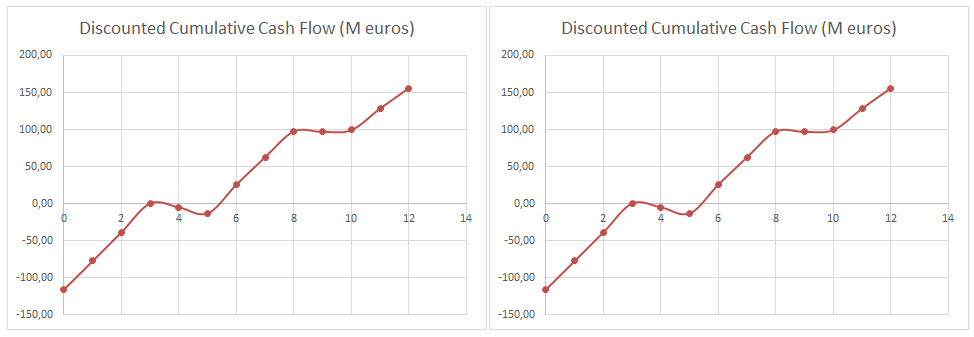
\includegraphics[width=140mm]{CCFTogether.png}


\item Updated Pay Back Time. The Discounted Cumulative Cash Flow has already been plotted too. It can be seen that the Updated Pay Back Time is between 2 and 3 years. If again linearly distribution is assumed, the Updated Pay Back time will be of 2.99 years. This value seems reasonably acceptable, because of the nature of the project, within the space sector, a very demanding and expensive one.
This time, because of the significat costs during year 4 (building and assembling of satellites) and especially year 5 (re-launching of satellites), added to the fact that the discount rate is now being taken into account to, it makes the Discounted Cumulative Cash Flow negative again, as can be seen in the graphic. Therefore, there will be another Updated Pay Back Time for the inversion done during years 4 and 5, exactly at year 5.33. Taking into account that this inversion was made during the year 4, it turns out to be an actual UPBT of 1.33 years. There won't be a third UPBT. In years 9 and 10 there is a big investment again, but by then, the profit is high enough so as to make it possible for the Discounted Cumulative Cash Flow to not become negative any more. 


\item Break Even Point. By changing manually the parameter "Number of Mbits hired" of first year, it is found that the Break Even Point is of 18375000 Mbits (with this value of Mbits hired the first year, the Cash Flow is approximately 0). This means that under no account there can be less Mbits hired that that, because otherwise the Cash Flow would be negative and the Cumulative Cash Flow, negative at beginning since first year is fully just invest, would never reach a positive value, generating losses. From the assumptions of demand already explained, it can be seen that having a greater demand than the BEP is very likely to happen. Thus, the cash flow will be positive and consequently there will be a time in which there is benefit.

\item Net Present Value. From the table, it can be immediately seen that the Net Present Value (for the period of time studied, of 12 years) is of +156.01M\euro. The Net Present Value is the difference between the present value of cash inflows and the present value of cash outflows over a period of time. It is clearly positive, which indicates that the project earnings generated by the investment exceeds the costs. In other words, it will be profitable. The Net Present Value coincides with the value of the Discounted Cumulative Cash Flow of the twelfth year. 


\item Internal Rate of Retorn. The internal rate of retorn is the interest rate at which the Net Present Value of all the cashflows is equal to zero. This is used to evaluate the attractiveness of a project. If the Internal Rate of Return of a project exceeds a company's required rate of return, the project is desirable, and if on the other hand the IRR falls below the required rate of return, the project should be rejected. The studied carried on uses a 6\% as the discount rate, and this value gives a positive Net Present Value, as has been already explained. By manually changing the discount rate, it can be achieved that the Net Present Value gets to 0, or very closely. This value of the discount rate is the Internal Rate of Return, and is used to evaluate the attractiveness of a project. In this case, it has been found that the IRR is of 26.80\%. The higher the IRR is, the more desirable is to undertake the proeject. In any case, it must be greater than the actual discount ratio. In this case, not only the IRR is greater, but it is actually a very high rate. Therefore, the project is very attractive, feasibly speaking. 

\end{itemize}


The Pay Back Time and the Updated Pay Back Time are of approximately 3 years, quite acceptable in the space sector. The Net Present Value is really great, as well as the Internal Rate of Return. Moreover, the estimation of demand is far higher than the Break Even Point. In conclusion, all the parameters analysed happen to indicate the same thing: the investment is strongly recommended and the project is feasible. Nevertheless, it must not be forgotten than this study is done upon some important assumptions, which provide a certain degree of uncertainty. Nonetheless, the results of the study have been so positive that a slight variation of the hypothesis done could not lead to a unfeasible situation. 
